\chapter{Sviluppo del progetto}
\label{cap:sviluppo-progetto}
%In questo capitolo verrà descritto lo scopo di questo progetto, i requisiti necessari al suo raggiungimento e i dettagli della sua struttura interna che ne permette il funzionamento. \\
%In particolare andremo ad analizzare i class diagram che mostrano le relazioni tra le classi che li costituiscono e discuteremo delle scelte implementative fatte.

%\section{Obiettivo e requisiti}

L'obiettivo di questa tesi è realizzare un programma in linguaggio Java che sia in grado di ricevere in ingresso la struttura del modello descritta in linguaggio XML e di scrivere in modo automatico il codice NetLogo che possa eseguire la simulazione di interesse, rendendo, quindi, trasparente il processo di scrittura del codice.\\
%
Questo progetto è costituito da una struttura composita centrale di classi in cui vengono conservate tutte le informazioni necessarie per l'esecuzione della simulazione. Come mostrato nel Paragrafo \ref{sec:strttura-interna} l'oggetto di tipo Graph che rappresenta la struttura è composto da classi che modellano la topologia dell'ambiente e da classi che rappresentano i comportamenti da simulare.\\
L'informazione conservata in questa struttura viene estratta da un apposito parser che implementa il pattern Builder per la costruzione e composizione degli oggetti.\\
Infine si è implementato il pattern Visitor per visitare gli oggetti della struttura e generare il relativo codice NetLogo.\\
%
I modelli NetLogo che vengono generati da questo componente sono costituiti da un ambiente fisico modellato sotto forma di grafo con nodi e archi che rappresentano rispettivamente incroci e strade, caratterizzati da coordinate spaziali e dimensioni fisiche. In questo ambiente si muovono attori che possono avere comportamenti differenti. Nel nostro caso abbiamo deciso di modellare i comportamenti degli attori come una lista di punti di interesse che questi devono visitare prima di poter uscire.\\
%
Nei paragrafi che seguono, dopo aver descritto tutte le componenti che costituiscono questo progetto, andiamo a delineare la struttura dei documenti XML previsti e dei modelli NetLogo generati. Infine nel Paragrafo \ref{sec:requisiti} si descrivono le librerie usate .

\section{Struttura centrale}
\label{sec:strttura-interna}
L'unico scopo delle classi Java utilizzate è quello di rappresentare e conservare l'informazione raccolta dal documento XML, senza eseguire alcun tipo di manipolazione. Per questo motivo abbiamo cercato di mantenere la struttura delle classi il più semplice possibile, come mostrato in Figura \ref{fig:graph-diagram}.\\
La classe Graph è caratterizzata da una composizione di Edge, Node e Behavior. Espone metodi per il recupero delle informazioni e per la validazione di nodi e archi, in modo tale da impedire l'aggiunta di nodi nella medesima posizione e di archi con gli estremi uguali.\\ 
\begin{figure}[htbp]
\centering
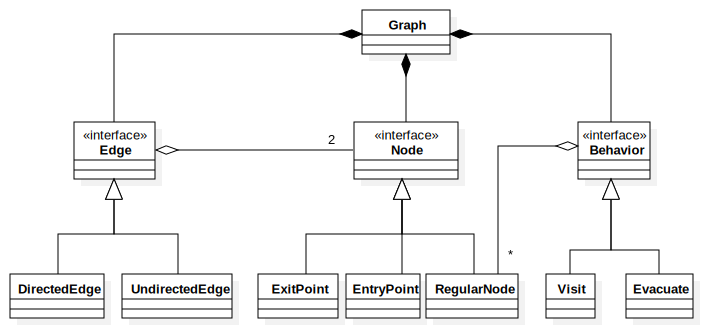
\includegraphics[width=\textwidth,height=\textheight,keepaspectratio]{images/graph-diagram.pdf}
\caption{Class diagram della struttura del grafo}
\label{fig:graph-diagram}
\end{figure}
Ogni behavior è caratterizzato da un identificatore, attribuitogli dall'XML e da una lista di nodi regolari di interesse che devono essere visitati prima di permettere all'attore di puntare ad una uscita.\\
Gli edges in questo modello sono aggregazioni di due nodi e presentano un particolare attributo “weight” che verrà usato dalle funzioni NetLogo per la generazione dei percorsi a costo minimo.\\
Infine ogni classe che implementa l'interfaccia Node, oltre ai metodi per il recupero delle informazioni conservate, implementa anche un metodo statico per il controllo dei parametri, in modo tale da impedire la costruzione di nodi con informazioni incompatibili con NetLogo.

\section{Parser XML}
\label{subsec:parser-builder}
Come già accennato, abbiamo scelto il formato JDOM per la rappresentazione del file XML. La scelta di questo formato è stata dettata dalla sua struttura, che si adatta meglio ai nostri fini di sola lettura e non di manipolazione del documento.\\
La struttura ad albero del modello generato rispecchia il documento XML. Ogni nodo dell'albero è di tipo \texttt{Element} e conserva una lista dei figli e un riferimento al padre, espone inoltre una ricca interfaccia con cui si possono estrarre tutte le informazioni di interesse come gli attributi associati al tag rappresentato, oppure il testo sottostante.\\
Il parser XML inoltre esegue controlli mirati a verificare che siano fornite tutte le informazioni necessarie all'esecuzione del modello NetLogo.\\
\begin{figure}[htbp]
\centering
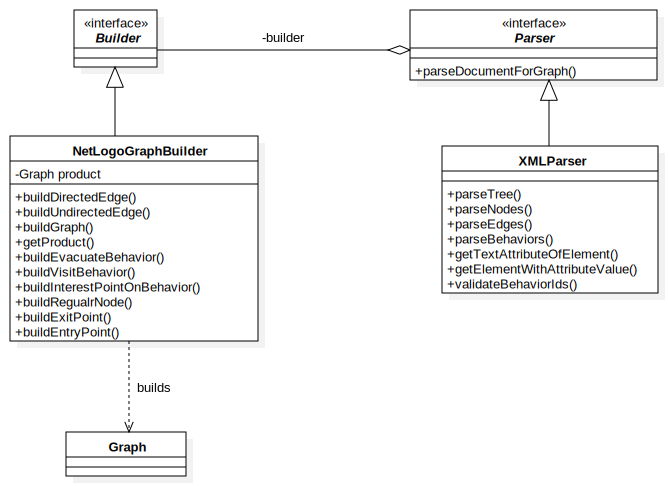
\includegraphics[width=\textwidth,height=\textheight,keepaspectratio]{images/builder-diagram.pdf}
\caption{Class diagram di Parser e Builder}
\label{fig:builder-diagram}
\end{figure}
\section{Builder}
Per la costruzione delle classi abbiamo usato il pattern Builder, in modo da mantenere il processo di costruzione della struttura interna dell'oggetto di tipo Grafo trasparente all'utente di questo strumento. In particolare l'interfaccia del Builder aiuta a mantenere l'algoritmo di interpretazione dell'XML separato dal processo di costruzione e rappresentazione del suo contenuto in classi Java.\\
Il pattern Builder, inoltre, porta il grande beneficio di migliorare la modularizzazione derivante dall'incapsulamento di tutta la procedura di manipolazione della struttura interna dell'oggetto costruito, in questo modo il Client non ha necessità di conoscere la sua composizione interna.\\
Una conseguenza che rende il pattern ancora più adatto al nostro caso è il miglioramento del controllo sul processo di costruzione del prodotto. Al contrario di altri pattern creazionali, i quali costruiscono e restituiscono il prodotto in un'unica funzione, il Builder separa queste due operazioni mettendo a disposizione un'interfaccia più completa.\\
Grazie a questo noi siamo in grado di esercitare un maggiore controllo sulla correttezza delle operazioni eseguite e delle informazioni inserite durante questa prima fase.\\
L'interfaccia Parser rende il progetto aperto ad estensioni future, come il supporto di linguaggi alternativi all'XML.\\
\begin{figure}[htbp]
\centering
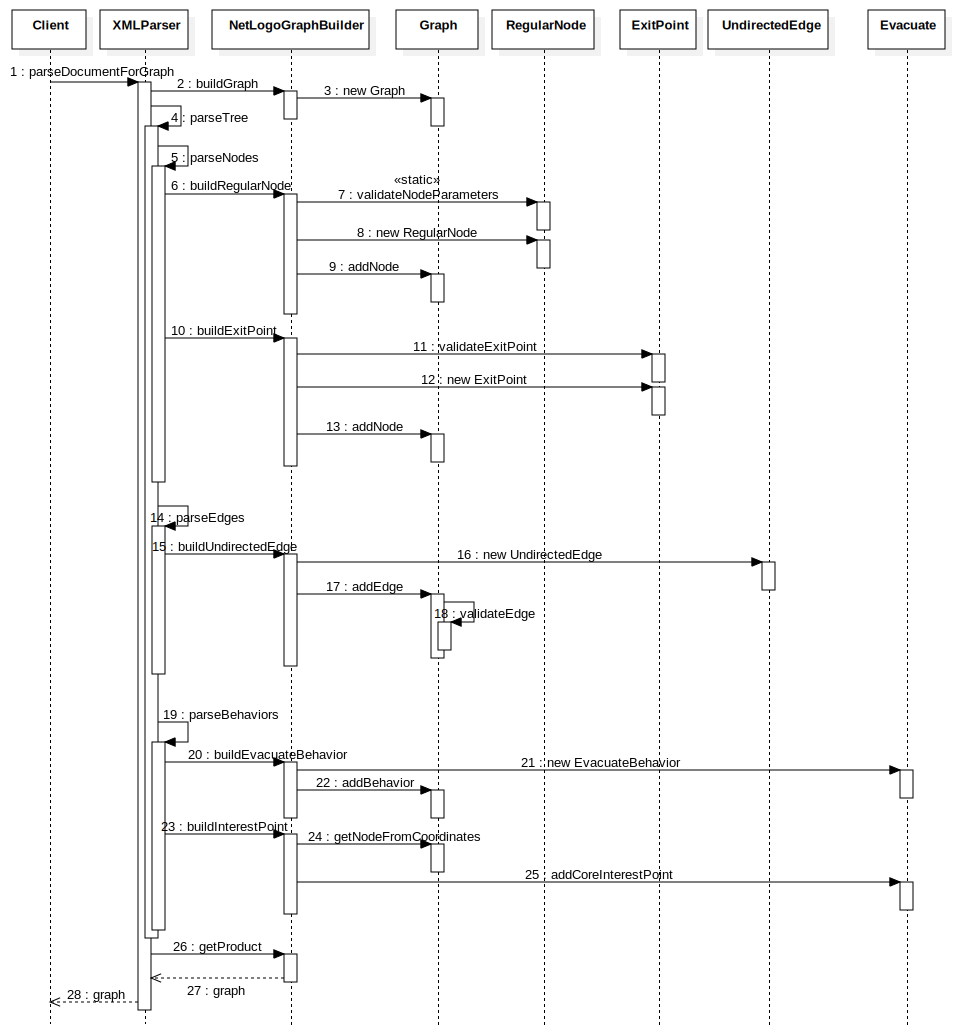
\includegraphics[width=\textwidth,height=\textheight,keepaspectratio]{images/builder-sequence.pdf}
\caption{Sequence diagram della costruzione di un grafo da parte di XMLParser}
\label{fig:builder-sequence}
\end{figure}
%Come si vede in Figura \ref{fig:builder-diagram} il parser esercita il ruolo di Director per il builder. Il processo di analisi del documento e costruzione degli oggetti Java è descritto nel sequence diagram in Figura \ref{fig:builder-sequence}.\\
Come si può osservare in Figura \ref{fig:builder-diagram} e \ref{fig:builder-sequence} la classe \texttt{XMLParser} svolge il ruolo di \textit{Director} all'interno del pattern e, durante la visita della struttura JDOM creata, chiama i metodi del \textit{Builder concreto} \texttt{NetLogoGraphBuilder} per la costruzione dei vari oggetti. Quest'ultimo, prima di procedere alla costruzione dell'oggetto e al suo inserimento nella struttura, esegue controlli sulla correttezza delle informazioni estratte dal parser.\\
Quando la visita da parte del parser è conclusa viene recuperato il \textit{Product}, che non è altro che un oggetto di tipo \texttt{Graph}.

\section{Visitor}
\label{subsec:visitor}
Per l'operazione di scrittura del codice NetLogo si ha la necessità di estrapolare dagli oggetti che costituiscono la struttura del grafo diverse informazioni. Al variare della classe concreta varieranno anche le informazioni specifiche da estrarre.\\
Il grafo inoltre presenta una struttura di classi con interfacce diverse che devono, quindi, essere modificate per poter eseguire l'operazione necessaria.\\
In questo contesto, quindi, il pattern Visitor si rivela molto utile permettendo di eseguire operazioni specifiche al variare della classe concreta senza inquinare le diverse interfacce all'interno della struttura.\\
Un ulteriore vantaggio presentato dal Visitor è quello di concentrare le funzioni per la scrittura del codice NetLogo in classi specifiche rendendo il sistema più facile da manutenére ed eventualmente estendere.\\
La struttura dei modelli NetLogo finali è tale che gran parte del codice necessario rimane fissa al variare della simulazione, per questo motivo si ha che l'operazione di scrittura del codice NetLogo eseguita dai visitor è alternata a quella di lettura da appositi file di testo che contengono la parte fissa del modello. Queste parti fisse quindi vengono completate con le informazioni estrapolate dagli oggetti Java precedentemente messi in vita.\\
Abbiamo inoltre scelto di separare il modello NetLogo finale in due parti, mantenendo distinta la parte del modello che mette in vita l'ambiente da quella che controlla i movimenti degli attori e raccoglie le informazioni di interesse.\\
\begin{figure}[htb]
\centering
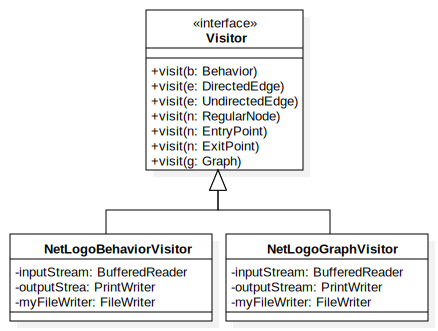
\includegraphics[width=\textwidth,height=\textheight,keepaspectratio]{images/visitor-class-diagram.pdf}
\caption{Class Diagram del Visitor}
\label{fig:visitor-diagram}
\end{figure}
Si hanno quindi due classi visitor distinte per ognuno dei due modelli NetLogo da creare: NetLogoGraphVisitor e NetLogoBehaviorVisitor ( Figura \ref{fig:visitor-diagram} ). Il primo effettua una visitita su nodi e archi del grafo per scrivere i comandi necessari a mettere in vita l'ambiente corretto. Il secondo, invece, effettua una visita sui behaviors in modo da definire i comportamenti che gli attori potranno avere nella simulazione e sui nodi per impostare lo stato iniziale del sistema.\\
In questo modo le interfacce delle classi del grafo, rimangono inalterate ma le operazioni effettuate variano al variare del visitor concreto, rendendolo un pattern ancora più adatto a questo specifico caso.\\
In Figura \ref{fig:visitor-sequence} è mostrato il funzionamento di un NetLogoGraphVisitor. L'oggetto finale ottenuto da questo visitor è un file eseguibile \texttt{.nlogo} in cui viene costruito l'ambiente con la corretta topologia e viene esportato un file di stato del modello nel formato \texttt{.csv} necessario al secondo modello per l'acquisizione dell'ambiente.\\
\begin{figure}[htbp]
\centering
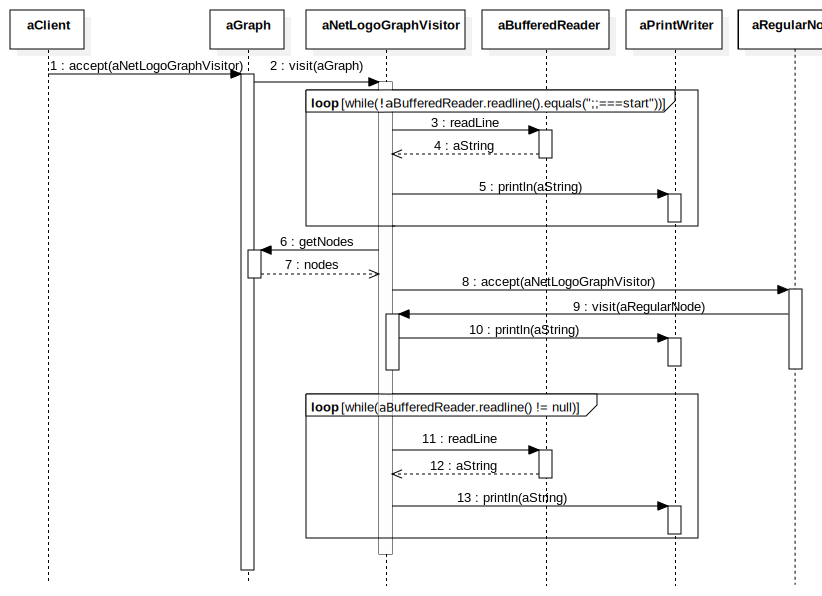
\includegraphics[width=\textwidth,height=\textheight,keepaspectratio]{images/visitor-sequence.pdf}
\caption{Sequence Diagram del NetLogoGraphVisitor su un grafo con un unico nodo}
\label{fig:visitor-sequence}
\end{figure}
NetLogoBehaviorVisitor, in modo analogo, eseguirà operazioni di lettura e scrittura alternate per generare un un secondo file \texttt{.nlogo} in cui si esegue la simulazione e si esportano i dati di interesse.

\begin{figure}[htbp]
\centering
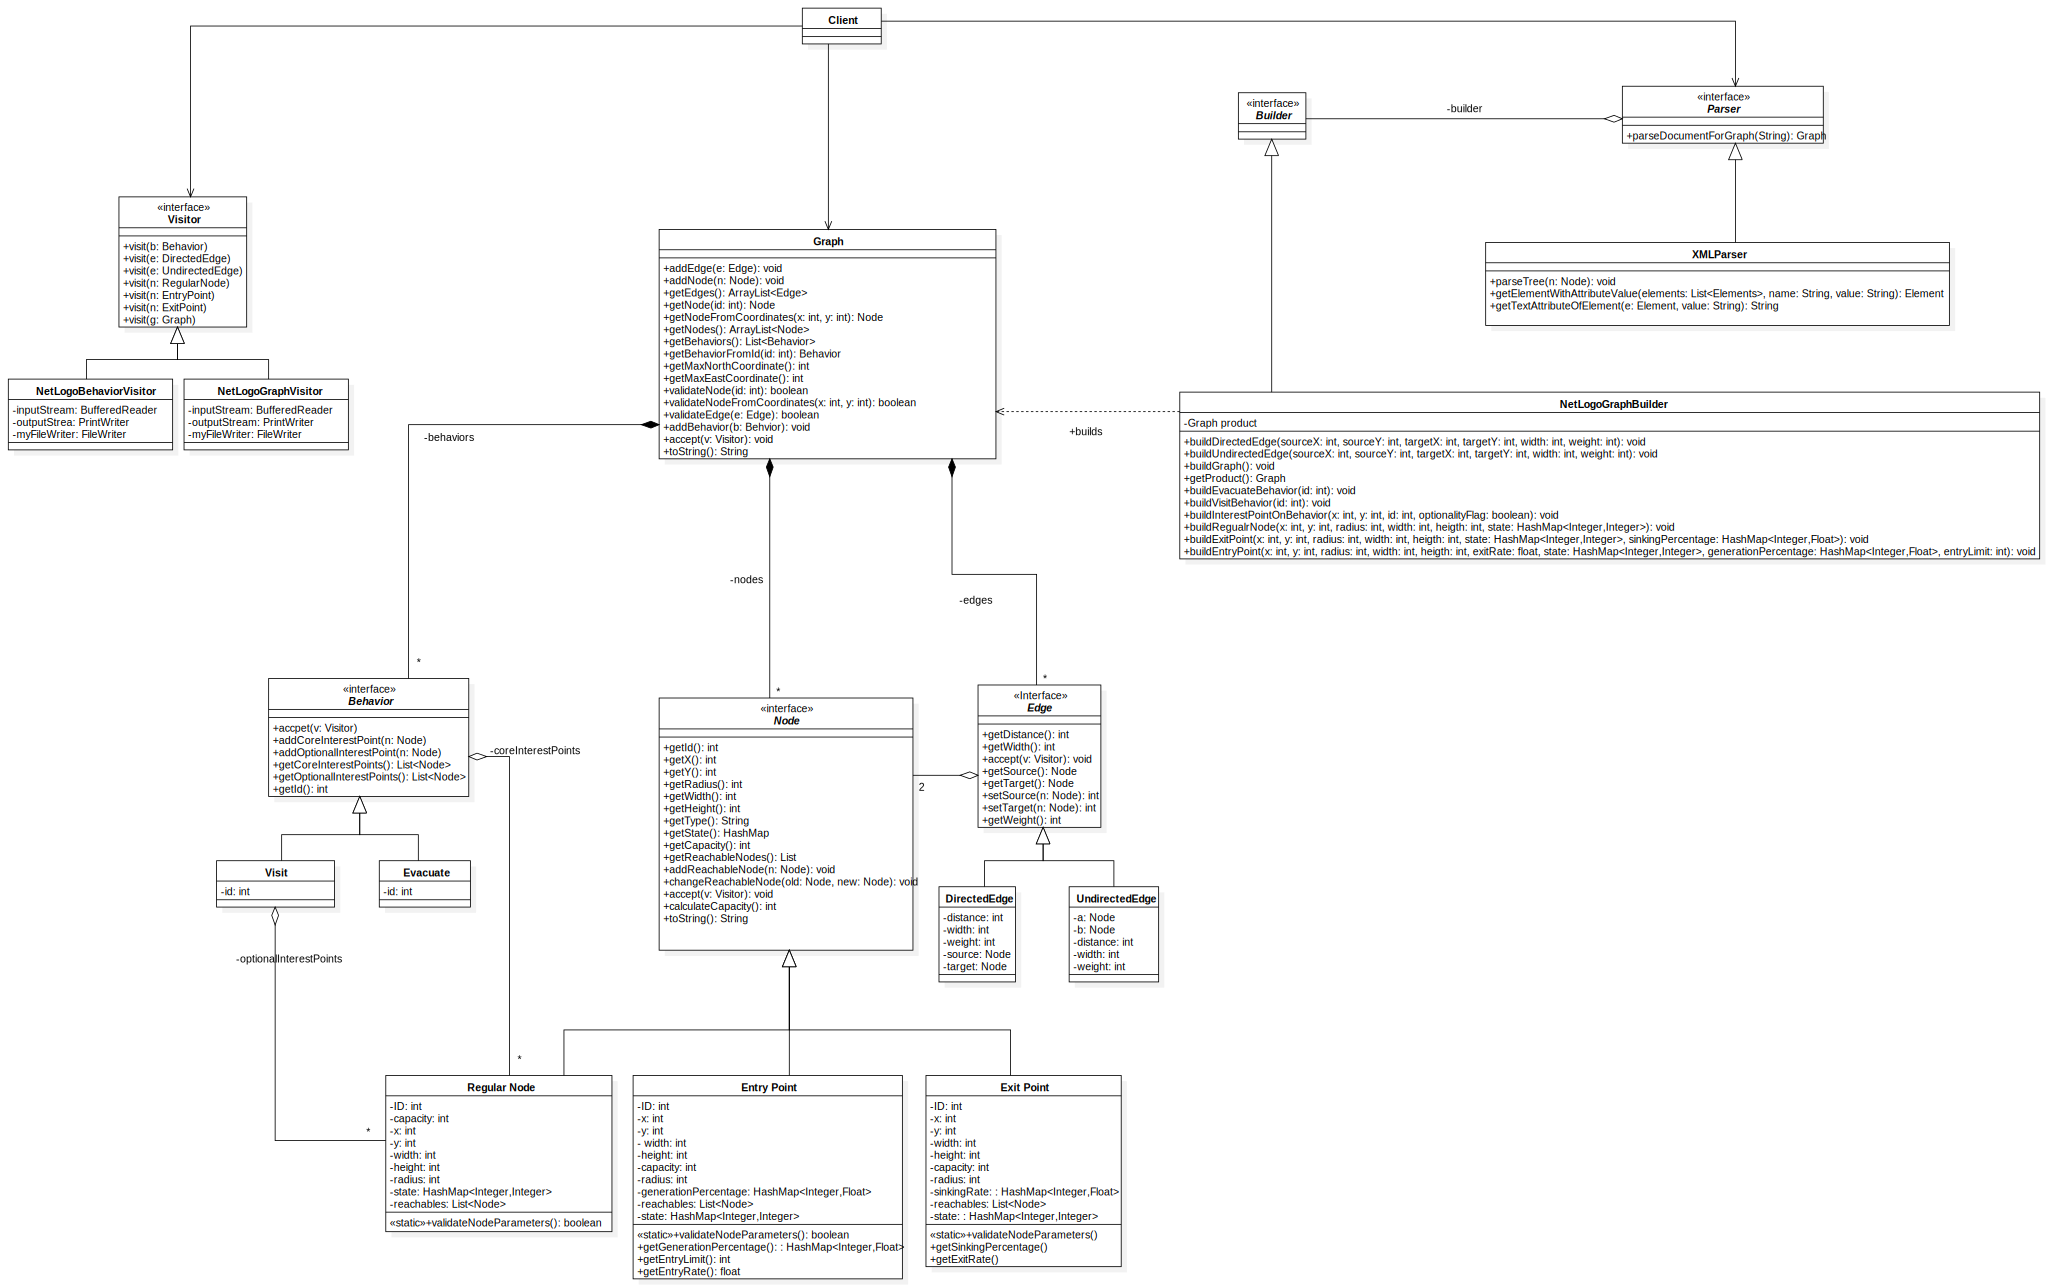
\includegraphics[width=\textwidth,height=\textheight,keepaspectratio]{images/complete-diagram.pdf}
\caption{Classi diagram}
\label{fig:complete-diagram}
\end{figure}

\section{Documento XML}
La struttura del documento XML prevista per il funzionamento del nostro strumento si attiene il più possibile allo standard di formato GraphML \cite{graphml} (approvato dal W3C) in modo da evitare inconsistenze e incomprensioni, soprattutto per la parte in cui è descritta la topologia dell'ambiente, per la quale questo formato è pienamente adatto.\\
Il file XML è suddiviso in tre sezioni distinte:
\begin{itemize}
\item \texttt{Graph}
\item \texttt{Behaviors}
\item \texttt{System}
\end{itemize} 
\texttt{Graph} rappresenta la topologia dell'ambiente in cui gli attori si muovono, ed è descritta sotto forma di grafo con \texttt{edges} che rappresentano le strade e \texttt{nodes} che rappresentano gli incroci.\\
Gli edges possono essere \texttt{directed} e \texttt{undirected}, per ognuno di essi vengono specificati peso e larghezza, ovvero \texttt{weight} e \texttt{eWidth}. Il formato GraphML, inoltre, permette di specificare un tipo di default per gli edges come valore dell'attributo \texttt{edgedefault} di Graph.\\
I nodes invece possono essere di tre tipi: normal, entry o exit. Per tutti e tre i tipi vengono specificate coordinate spaziali e dimensioni fisiche dell'incrocio che esso rappresenta, quindi avremo \texttt{nx}, \texttt{ny}, \texttt{nWidth}, \texttt{nHeight} e \texttt{nRadius}. All'interno del codice si usa l'attributo \texttt{ntype} per specificare il tipo di nodo e anche in questo caso è possibile specificare un tipo di default settato a \texttt{normal}.\\
Per quanto riguarda i \texttt{Behaviors} si ha una struttura a grafo in cui ogni nodo rappresenta un behavior di cui viene indicata la tipologia, ovvero \texttt{bType}, l'identificatore e la lista dei nodi di interesse.\\
La sezione \texttt{System} descrive lo stato iniziale dell'ambiente. Per questa parte del modello si è preferito distaccarci leggermente dallo standard, in modo da avere una struttura più comprensibile, usando gli specifici tag \texttt{<behavior \textbackslash>}. Per ogni nodo, sotto il tag “\texttt{graph}” con identificatore \texttt{state}, viene indicato il comportamento e la quantità degli attori presenti. In particolare, nei nodi contrassegnati come entry o exit, vi è un ulteriore tag “\texttt{graph}” con identificatore \texttt{parameters} in cui si specificano la frequenza di generazione o eliminazione degli attori e le percentuali relative ad ogni behavior. Per i nodi di ingresso viene anche indicato un limite superiore agli attori generabili (\texttt{entry-limit}), che può essere messo negativo nel caso in cui, invece, non si vogliano porre limiti.

\subsection{Esempio}
Di seguito è riportato un XML in cui si mostra la definizione di ogni tipo di entità coinvolta: attributi, tutti i tipi di nodi, tutti i tipi di archi, behavior e stato associato ai nodi.

\definecolor{darkgreen}{rgb}{0,0.5,0}

\lstdefinelanguage{XML}{
  basicstyle=\linespread{1.1}\ttfamily,
  morestring=[s]{"}{"},
  morecomment=[s]{!--}{--},
  commentstyle=\color{blue},
  moredelim=[s][\color{black}]{>}{<},
  moredelim=[s][\color{violet}]{\ }{=},
  stringstyle=\color{red},
  identifierstyle=\color{darkgreen},
  tabsize=2,
  breaklines=true,
  breakatwhitespace=true
}

%\lstinputlisting[language=XML, firstline=0, lastline=6]{images/example.xml}
%\[\textbf{[...]}\]
%\lstinputlisting[language=XML, firstline=30, lastline=45]{images/example.xml}
%\[\textbf{[...]}\]
%\lstinputlisting[language=XML, firstline=53, lastline=69]{images/example.xml}
%\[\textbf{[...]}\]
%\lstinputlisting[language=XML, firstline=77, lastline=124]{images/example.xml}
%\[\textbf{[...]}\]
%\lstinputlisting[language=XML, firstline=135, lastline=155]{images/example.xml}

\lstinputlisting[language=XML, firstline=0, lastline=6]{images/example.xml} %attributi
\[\texttt{[...]}\]
\lstinputlisting[language=XML, firstline=30, lastline=38]{images/example.xml} %nodo regolare
\[\textbf{[...]}\]
\lstinputlisting[language=XML, firstline=152, lastline=169]{images/example.xml} %entry e exit node
\[\textbf{[...]}\]
\lstinputlisting[language=XML, firstline=178, lastline=188]{images/example.xml} %edges
\[\textbf{[...]}\]
\lstinputlisting[language=XML, firstline=297, lastline=318]{images/example.xml} %behavior e stato nodo regolare
\[\textbf{[...]}\]
\lstinputlisting[language=XML, firstline=439, lastline=469]{images/example.xml} %stato entry e exit
\[\textbf{[...]}\]
\lstinputlisting[language=XML, firstline=484, lastline=485]{images/example.xml} %chiusura tag


\section{Modello NetLogo}
Come già accennato in precedenza abbiamo scelto di dividere il modello NetLogo generato dal nostro programma in due parti con lo scopo di mantenere le funzioni necessarie per la costruzione dell'ambiente separate da quelle che modellano i movimenti degli attori e raccolgono le informazioni sulla simulazione eseguita. In questo modo il codice è più facile da gestire e manutenere.\\
Questa scelta porta, inoltre, il vantaggio di eseguire il primo modello una vola sola e di sfruttare, invece, il file di stato che esso genera nel caso in cui si vogliano simulare le interazioni di diversi comportamenti nello stesso ambiente.
\subsection{Ambiente}
L'ambiente in cui gli attori si muoveranno è modellato sotto forma di grafo con specifiche tipologie di turtles dette \texttt{beacon} che fanno da nodi e rappresentano quindi gli incroci tra le vie percorribili.\\
Gli archi sono rappresentati da due tipologie diverse di turtles dette \texttt{street}, percorribile in entrambi i versi, e \texttt{directed-street}, percorribile solo in un verso.\\
\begin{figure}[htbp]
\centering
\includegraphics[width=\textwidth,height=\textheight,keepaspectratio]{images/ambiente-screen.png}
\caption{Esempio di ambiente generato. In questo caso i beacons di ingresso sono di colore blu e i beacons di uscita di colore rosso.}
\label{fig:ambiente-screen}
\end{figure}
Per i beacons di ingresso e di uscita vengono anche impostati i relativi parametri, ovvero tasso di generazione o eliminazione degli attori e percentuali relative ai behavior da attribuire ad essi. In particolare per gli entry points si imposta anche un limite massimo del numero di attori che possono essere generati.\\
Grazie a questi parametri il sistema è predisposto per lo studio di simulazioni in ambienti comunicanti, in cui quindi gli attori possono uscire da un ambiente e entrare in un altro. 
\subsection{Behaviors e stato iniziale}
Abbiamo scelto di caratterizzare i behaviors degli attori con un identificatore intero e una lista di nodi di interesse che l'attore deve raggiungere prima di uscire dall'ambiente.\\
Sono state inoltre inserite due possibili modalità di raggiungimento dei beacons di interesse: ”\texttt{minDistance}” e “\texttt{orderedList}”. Nella prima l'attore punta al nodo più vicino a quello precedentemente raggiunto tra quelli di interesse, nella seconda invece la lista viene rigidamente percorsa rispettandone l'ordine.\\
Lo stato iniziale del sistema è contenuto in una semplice lista \texttt{initial-state} che viene percorsa da una apposita funzione per la corretta generazione degli attori sui vari nodi. 
\begin{figure}[htbp]
\centering
\includegraphics[width=\textwidth,height=\textheight,keepaspectratio]{images/movers-screen.png}
\caption{Esempio di ambiente popolato con attori nello stato iniziale. Gli attori hanno assunto il colore del beacon che hanno come obiettivo, in questo caso abbiamo un unico behavior che ha come interest point il beacon di colore verde.}
\label{fig:movers-screen}
\end{figure}

\section{Requisiti}
\label{sec:requisiti}
La scelta del linguaggio XML è dettata dalla sua diffusione, con lo scopo di ridurre le conoscenze preliminari necessarie per l'utilizzo di questo strumento e per facilitare la sua integrazione con altri componenti.\\
Per l'analisi del documento XML esistono diverse alternative, tra le quali le più interessanti sono: DOM, SAX e JDOM.\\
DOM (Document Object Model) è uno standard cross-platform e language-indipendent stabilito dal W3C per la rappresentazione di documenti strutturati, quindi XML, HTML, XHTML, come modelli orientati agli oggetti. Il difetto di questo formato e delle sue API, però, sta nella pesantezza in memoria.\\
La tecnologia SAX (Simple Api for Xml) rappresenta un'alternativa veloce e potente nel caso in cui si voglia gestire il documento con un approccio event-driven.\\
JDOM \cite{jdom}, infine, è un formato open-source disegnato appositamente per Java che completa DOM e SAX semplificando la manipolazione dei documenti XML. Questo al contrario delle due alternative non è incluso nel JDK, ma è ampiamente accettato dalla comunità.\\
Il metodo più rapido e semplice per analizzare un documento XML e costruire un modello JDOM è attraverso le API SAX, che JDOM, grazie alla sua natura open source, può sfruttare.\\
La API JDOM2 associata al formato, quindi, usa la classe \texttt{SAXBuilder} \cite{sax-builder} per costruire il modello JDOM sotto forma di albero che rispecchia la struttura del documento da cui è stato estratto. 

%Ogni nodo dell'albero è di tipo \texttt{Element} e conserva una lista dei figli e un riferimento al padre, espone inoltre una ricca interfaccia con cui si possono estrarre tutte le informazioni di interesse come gli attributi associati al tag rappresentato, oppure il testo sottostante.\\

Per quanto riguarda la parte della scrittura del codice NetLogo, si ha che gran parte del codice che modella la simulazione rimane fissa al variare dei modelli descritti negli XML, quindi abbiamo pensato di mantenere questa in un semplice file di testo che viene letto e integrato con le informazioni contenute negli oggetti Java. Per le operazioni di lettura e scrittura su file abbiamo usato le classi \texttt{BufferedReader} \cite{buffered-reader} e \texttt{PrintWriter} \cite{print-writer} che permettono lettura e scrittura di intere linee di testo.\\ 

Lo strumento segue il seguente workflow:
\begin{itemize}
\item analisi del documento XML e costruzione di una rappresentazione della struttura orientata agli oggetti in JDOM attraverso la relativa API;
\item costruzione degli oggetti Java per la rappresentazione della simulazione descritta nel modello JDOM;
\item visita degli oggetti Java e scrittura su file del codice NetLogo che eseguirà la simulazione.
\end{itemize}
